\section{The Z-Wave Device API Data model}
\label{datamodel} 
 
Z-Way holds all data of the Z-Way network  in a data holder structure. The data holder 
structure is a hierarchical tree of data elements.  

Following the object-oriented software paradigm the different commands targeting the 
network or individual devices are also embedded into the data objects as object methods.
 
Each data element is handled in a data object that contains the data element and some contextual data.

\subsection{The Data object}
 
Each Data element such as devices[nodeID].data.nodeId is an object with the following child elements:
\begin{itemize}
\item value: the value itself
\item name: the name of the data object
\item updateTime: timestamp of the last update of this particular value
\item invalidateTime: timestamp when the value was invalidated by issuing a Get command 
to a device and expecting a Report command from the device
\end{itemize}

Every time a command is issued that will have impact on a certain data holder value the 
time of the request is stored in "invalidateTime" and the "updated" flag is set to "False". 
This allows to track when a new data value was requested from the network when this new 
data value was provided by the network.

This is particularly true if Z-Way is sending a SET command. In this case the data value 
is invalidated with the "SET" commands and gets validated back when the 
result of the GET command was finally stored in the data model.

To maintain compatibility with Javascript the data object has the following methods implemented

\begin{itemize}
\item valueOf(): this allows to obmit .value in JS code, hence write as an example data.level = 255
\item updated(): alias to updateTime
\item invalidated(): alias to invalidateTime
\end{itemize}

These aliases are not enumerated if the dataholder is requested (data.level returns 
{value: 255, name: "level", 
updatedTime: 12345678, invalidatedTime: 12345678}).


\begin{figure} 
\begin{center}
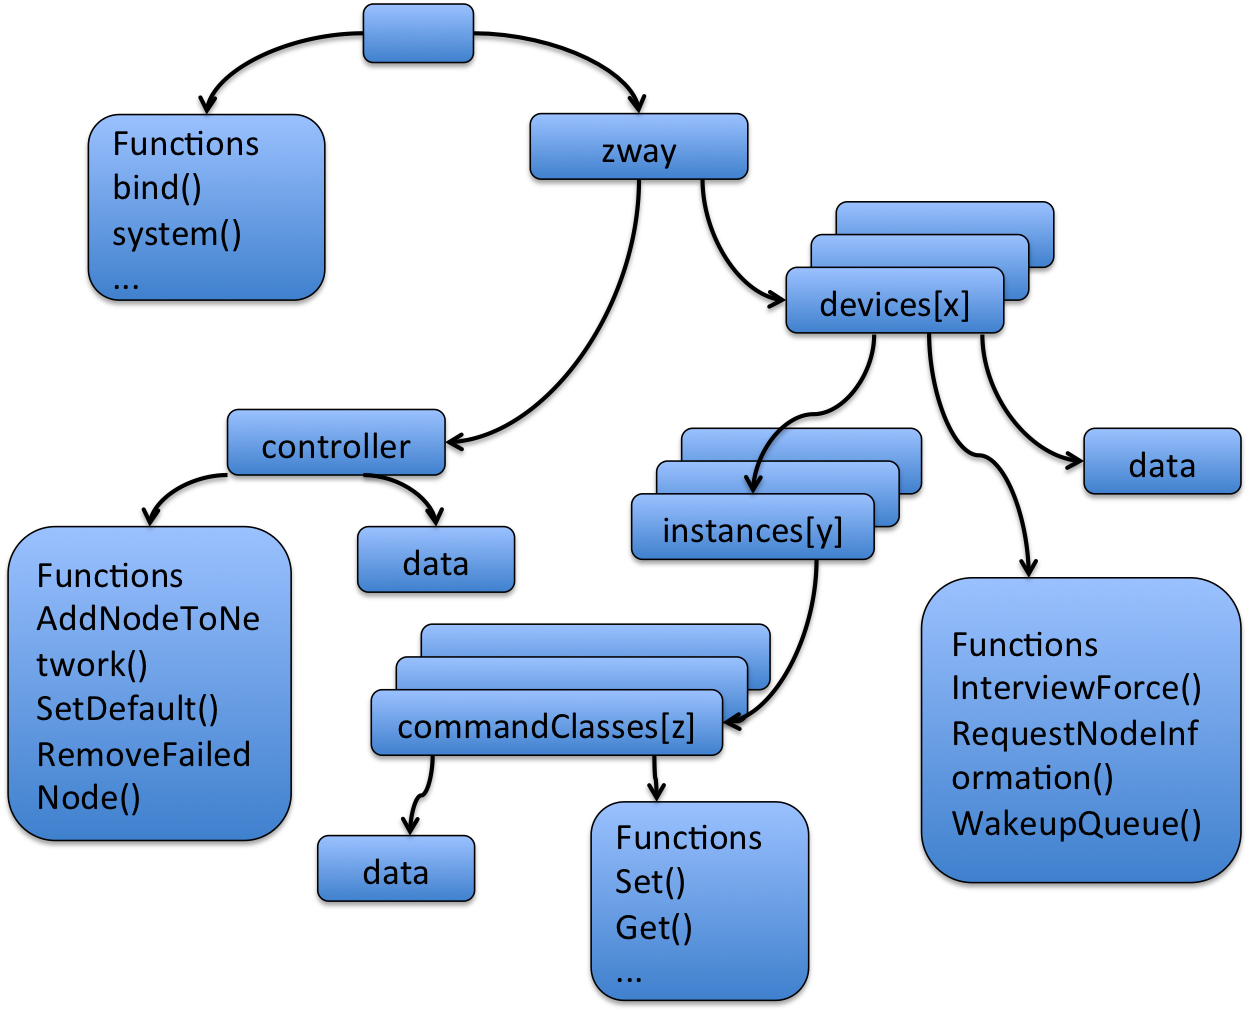
\includegraphics[scale=0.6]{pics/zwayblocks.png}
\caption{Z-Way Object Tree Structure}
\label{zwaystructure} 
\end{center} 
\end{figure} 
 
\subsection {The Data and Method Tree}
 
The root of the data tree has two important child objects:
\begin{itemize}
\item controller, this is the data object that holds all data and methods (commands,  mainly function classes) 
related to the Z-Way controller as such
\item devices array, this is the object array that holds the device specific data and methods (commands, 
mainly command classes). 
\end {itemize}

Chapter \ref{datamodel} gives a complete overview of the data and method tree.

\subsection {Device Data Visualization}

\begin{figure} 
\begin{center}
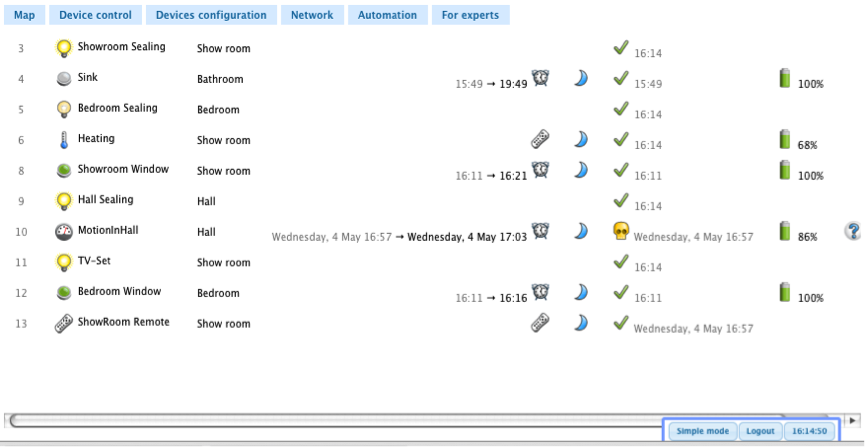
\includegraphics[scale=0.8]{pics/devicestatus.png}
\caption{Demo UI Dialog for Device Status}
\label{c4:demostatus} 
\end{center}
 \end{figure}
 
One example how to use the Data in the object tree is the device status page provided by 
the demo user interface in tab "Device Control" of the Expert UI.

 This tab gives an overview of the network status and the availability of each device. It shows the time stamp of the 
 last interaction between the controller  and the device. For battery powered devices the battery charging status, 
 the time of the last wakeup and the estimated time for the next wakeup is shown.
An info icon indicates when the interview of a device was not completed. Clicking on this device opens a window 
showing the interface status by command class. 
Please refer to the manual section “Interview” for more information about the interview process.

\begin{figure} 
\begin{center}
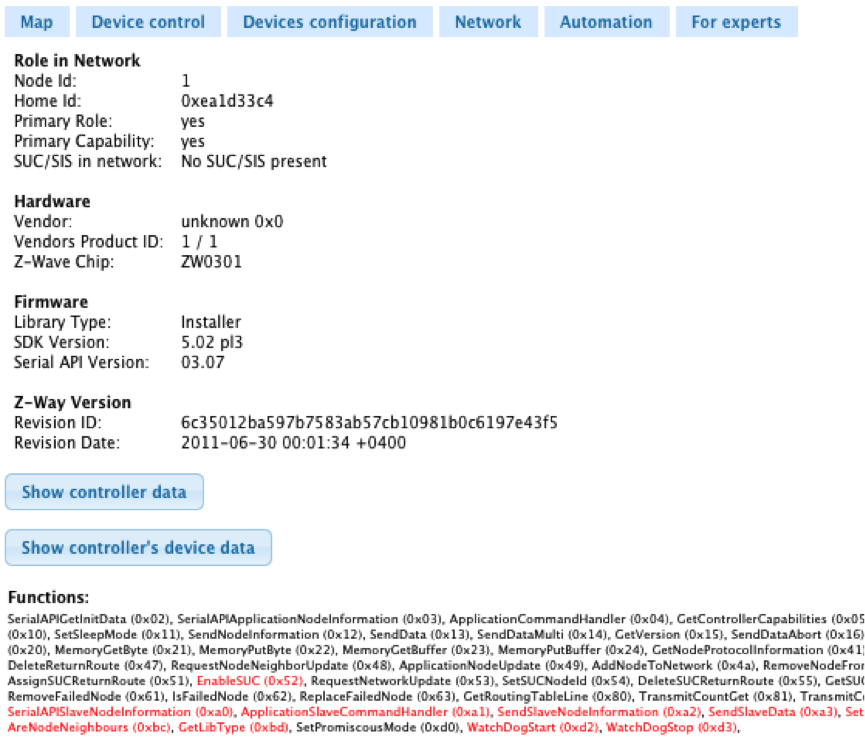
\includegraphics[scale=0.8]{pics/controllerstatus.png}
\caption{Demo UI Dialog for Controller information}
\label{c4:democontroller} 
\end{center}
 \end{figure}
  
The controller information tab shows all controller information. The buttons “Show Controller Data” shows the 
internal Z-Way data structure related to the specific controller function of the controller device. The button 
“Show controller device data” show the generic device related data of the controller device.

The information given on this page is only relevant for advanced Z-Wave developers and for debugging.

\subsection{Commands to control Z-Way itself} 
 
The last set of commands and values are not related to the Z-Wave network or the Z-Wave devices but to Z-Way itself.  
Chapter \ref{datamodel} lists all the commands and the values.

\subsection{Job Queue Handling}

The Job handling system is the core and heart of Z-Way. It is managing the different Function class and command class calls 
to the Z-Wave network and dispatches incoming messages. Every communication with the Z-Wave transceiver is scheduled 
into a job and queued that it can transmitted over the serial hardware interface. The API allows to look into the work of the job queue. 
The demo UI shows the Job queue under Tab "Network" but in expert  mode only.

\begin{figure} 
\begin{center}
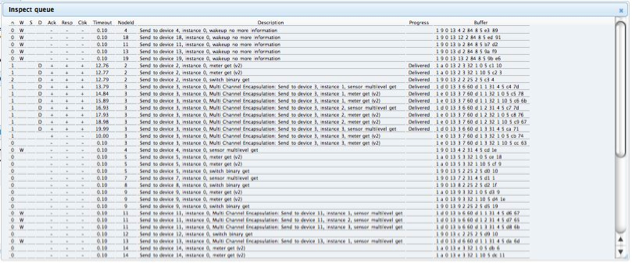
\includegraphics[scale=0.9]{pics/jobqueue.png}
\caption{Job Queue Vizualization in Demo UI}
\end{center} 
\end{figure}

The table shows the active jobs with their respective status and additional information.

\begin{table} 
\begin{tabular}{|p{0.3\textwidth}|p{0.6\textwidth}|} 
\hline
n	&This column shows the number of sending attempts for a specific job. Z-??Way tries three times to dispatch a job to the transceiver.\\ 
\hline 
W,S,D: & This shows the status of the job. If no indicator is shown the job is in active state. This means that the controller just tries to execute the job. 'W' states indicated that the controller believes that the target device of this job is in deep sleep state. Jobs in “'W' state will remain in the queue to the moment when the target devices announces its wakeup state by sending a wakeup notification to the controller. Jobs in 'S' state remain in the waiting queue to the moment the security token for this secured information exchanged was validated.
'D' marks a job as done. The job will remain in the queue for information purposes until a job garbage collection removed it from the queue.\\ 
\hline 
ACK:& shows if the Z-Wave transceiver has issued an ACK message to confirm that the message was successfully received by the transceiver. This ACK however does not confirm that the message was delivered successfully. A successful delivery of a message will result in a “D” state of this particular job.
If the ACK field is blank, then no ACK is expected. A “.” indicates that the controller expects an ACK but the ACK was not received yet. A “+” indicates that an ACK was expected and was received.\\ 
\hline
RESP	&shows if a certain command was confirmed with a valid response. Commands are either answered by a response or a callback.
If the RESP field is blank, then no Response is expected. A “.” indicates that the controller expects a Response but the Response was not received yet. A “+” indicates that a Response was expected and was received.\\ 
\hline
Cbk	&If the Cbk field is blank, then no callback is expected. A “.” indicates that the controller
expects a Callback but the Callback was not received yet. A “+” indicates that a Callback was expected and was received.\\
\hline 
Timeout	&Shows the time left until the job is de queued \\ 
\hline
Node Id	&shows the id of the target node. Communication concerning the network – like inclusion of new nodes – will have the controller node id as target node ID. For command classes command the node ID of the destination Node is shown. For commands directed to control the network layer of the protocol, the node id is zero. \\
\hline
Description	&shows a verbal description of the job \\
\hline
Progress	&shows a success or error message depending on the delivery status of the message. Since Z-Way tries three times to deliver a job up to 3 failure messages may appear.
Buffer: ... shows the hex values of the command sent within this job \\

\hline 
\end{tabular} 
\caption{Parameters of the Job Queue Vizualization} 
\label{c1:queuecommands} 
\end{table}

Table \ref{c1:queuecommands} summarizes the different values displayed on the Job Queue visualization. 
While these infos are certainly not relevant for end users of the system it is a great debug tool.  

